\section[Theoretische Grundlagen]{Theoretische Grundlagen\footcite[Theoretische Grundlagen basierend auf:\label{anleitung-ss2014}]
[]{anleitung-ss2014}}

\begin{sagesilent}
load('res/protokoll.sage')
\end{sagesilent}

\subsection{Einführung}
Im Versuch W1 wurde der Stirlingmotor als thermodynamische Maschine betrachtet. Mit Bezug auf den idealisierten thermodynamischen Stirling-Kreisprozess wurde versucht, das Verhalten des Motors zu erklären. Er wurde sowohl als Kältemaschine und Wärmepumpe (also mit Antrieb) als auch als Wärmekraftmaschine betrieben. Im ersten Fall wurden die Reibungsverluste beim Betrieb, die Kühlleistung (als Kältemaschine) und die Heizleistung (als Wärmepumpe), im zweiten Fall der Wirkungsgrad des Motors als Wärmekraftmaschine ohne Last (aus dem $(p, V)$-Diagramm) und unter Last (mithilfe des Pronyschen Zaums) bestimmt.

\subsection{Thermodynamische Größen}
In der Thermodynamik werden die Größen Temperatur $T$, innere Energie $U$ und Wärme $\Delta Q$ eingeführt. Die innere Energie ist die gesamte Energie eines Systems, insbesondere auch die durch die ungeordnete, mikroskopische Bewegung von Teilchen (Atome und Moleküle) beigetragene Energie. Die innere Energie kann sich nicht nur durch das Verrichten von Arbeit, sondern auch durch die Übertragung einer Energiemenge als Wärme ändern. Die Temperatur eines Körpers bestimmt dessen Fähigkeit, innere Energie in Form von Wärme abzugeben. Dabei gibt ein Körper höherer Temperatur immer Energie an einen Körper niedrigerer Temperatur ab, wenn beide in thermischem Kontakt stehen, bis schließlich beide dieselbe Temperatur haben.

Führt man einem Körper Wärme zu, erhöht sich dessen innere Energie und damit in der Regel auch die Temperatur:
\begin{equation}\label{eq:wärmekapazität}
\Delta Q = C_W \Delta T = c m \Delta T
\end{equation}
$C_W$ heißt Wärmekapazität, $c$ spezifische Wärme(kapazität). $C_W$ ist von der Masse $m$ des Körpers abhängig, während die spezifische Wärmekapazität $c$ massenunabhängig ist.
%Eine Wärmezufuhr von $\Delta Q$ führt zu einer proportionalen, von der Wärmekapazität abhängigen Änderung der Temperatur.
%Im Allgemeinen hängt $C_W$ selbst auch noch von der Temperatur ab.

\subsection{Zustandsgrößen und ideales Gas}
Ein thermodynamisches System kann vollständig durch Zustandsgrößen, deren Wert nicht von der "Vorgeschichte" des Systems abhängt, beschrieben werden. Hier sind hauptsächlich die Zustandsgrößen Druck $p$, Volumen $V$ und Temperatur $T$ wichtig.
%Zustandsgrößen werden wie folgt klassifiziert:
%\begin{description}
%\item[Extensive Größen:] Größen, die sich wie eine Menge verhalten und von der Größe des Systems abhängen. Dazu gehören u.a. Volumen $V$, Teilchenzahl $N$ und innere Energie $U$.
%\item[Intensive Größen:] Größen, die von der Größe des Systems unabhängig sind, aber ortsabhängig sein können. Der Druck $p$ und die Temperatur $T$ sind intensive Größen.
%\end{description}
Für ein ideales Gas (ein idealisiertes Modell, bei dem die Teilchen nur durch Stöße wechselwirken) gilt die folgende Zustandsgleichung:
\begin{equation}\label{eq:zustandsgleichung}
p V = N k_B T = n R T
\end{equation}
Dabei ist $N$ die Teilchenzahl bzw. $n$ die Teilchenzahl in \si{\mol}, $k_B = \SI{1,38e-23}{\J.\K^{-1}}$ die Boltzmann-Konstante und $R = \SI{8,315}{\J.\K^{-1}.\mol^{-1}}$ die universelle Gaskonstante.

Für eine feste Teilchenzahl enthält die Zustandsgleichung \cref{eq:zustandsgleichung} drei Variablen, wobei jeweils zwei den Wert der dritten festlegen.
%Allgemein kann das Verhalten einer Substanz in einem beliebigen Aggregatzustand (fest, flüssig, gasförmig) durch die Zustandsgleichung $p = p(V, T)$ charakterisiert werden.
%Man erhält also eine skalarwertige Funktion $p(V, T)$, die von zwei Veränderlichen abhängt.
%Diese Funktion
Die Zustandsgleichung
kann grafisch visualisiert werden, was in \cref{fig:zustandsfläche} gezeigt ist.
%Eine solche Visualisierung wird Zustandsfläche genannt.
"F", "Fl" und "G" kennzeichnen Bereiche, in denen die feste, flüssige bzw. gasförmige Phase vorliegt. $a$, $b$ und $c$ sind die Zweiphasengebiete F/Fl, Fl/G bzw. F/G. Die durchgezogenen Linien zeigen Isothermen (Kurven konstanter Temperatur), die gestrichelte eine Isobare (Kurve konstanten Drucks).

\begin{wrapfigure}[15]{l}{9.8cm}
	\centering
	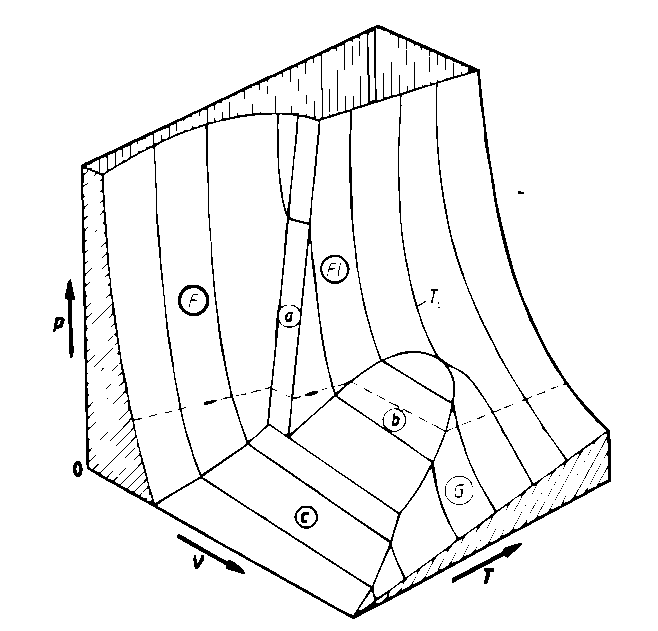
\includegraphics[scale=0.75]{res/Zustandsflaeche.pdf}
	\caption{Zustandsfläche eines einfachen Stoffs.\cref{anleitung-ss2014} \label{fig:zustandsfläche}}
\end{wrapfigure}

Wie schon in \cref{fig:zustandsfläche} zu sehen, haben Phasenübergänge für einen Stoff eine besondere Bedeutung. Um einen Stoff vom festen in den flüssigen oder vom flüssigen in den gasförmigen Zustand zu bringen, ist eine gewisse Wärmemenge, die Schmelz- bzw. Verdampfungswärme ($Q_S$ bzw. $Q_V$), auch latente Wärme genannt, nötig. Bei der umgekehrten Richtung wird diese Wärme wieder frei. Die tatsächlich benötigte Menge hängt von der Masse des Stoffs ab.
%\begin{equation*}
%	Q_{S/V} = m q_{S/V}
%\end{equation*}

%\subsection{Erster Hauptsatz der Thermodynamik}
%Der Energieerhaltungssatz muss in der Thermodynamik um die Energieform Wärme erweitert werden. Die innere Energie eines Stoffs kann sich nur ändern, wenn ihm durch Zu- oder Abfuhr von Wärme oder durch Verrichten von Arbeit Energie hinzugefügt oder entzogen wird. Dies ist der erste Hauptsatz der Thermodynamik:
%\begin{equation}\label{eq:hauptsatz}
%	\Delta U = \Delta W + \Delta Q
%\end{equation}
%Dabei bedeuten positive Größen, dass dem System Energie zugeführt wird, und negative, dass ihm Energie entzogen wird.

\subsection{Verrichtete Arbeit}
Bei einem thermodynamischen System bedeuten nach Konvention positive Größen, dass dem System Energie zugeführt wird, und negative, dass ihm Energie entzogen wird.

%Arbeit und Wärme sind keine Zustandsgrößen. Während der Wert der inneren Energie unabhängig davon ist, wie dem System diese Energie zugeführt wurde (durch Arbeit oder Wärme), kann z.B. bei einem Kreisprozess einer Maschine durch Zufuhr von Wärme Energie hinzugefügt werden, die diese durch Verrichten von Arbeit (z.B. indem Gas gegen einen Kolben expandiert) wieder abgeben kann. Nach jedem Umlauf (im ($p, V$)-Diagramm eine geschlossene Kurve) ist der Wert der inneren Energie unverändert, die Wärmemenge und verrichtete Arbeit hängen jedoch vom genauen Prozess und der Umlaufrichtung ab.

Um die verrichtete Arbeit explizit zu berechnen, wird folgende Überlegung angestellt: Expandiert ein Stoff um das Volumen $\Delta V = V_2 - V_1$ und bewegt dadurch (mit der Kraft $F$) einen Kolben der Fläche $A$ um den Weg $\Delta x = x_2 - x_1$, so wird die folgende Arbeit verrichtet:
\begin{equation}\label{eq:arbeit_allgemein}
	W = -\int_{x_1}^{x_2} F \diff x
	= -\int_{x_1}^{x_2} p A \diff x
	= -\int_{V_1}^{V_2} p(V, T) \diff V
\end{equation}
Dieser Zusammenhang ist für allgemeine Volumenänderungen gültig.
%  brauchen wir das?
%Für eine isotherme Zustandsänderung bei einem idealen Gas lautet das Ergebnis mit \cref{eq:zustandsgleichung}:
%\begin{equation}\label{eq:arbeit_isotherm}
%	W_\text{isotherm} = -\int_{V_1}^{V_2} \frac{N k_B T}{V} \diff V
%	= N k_B T \ln\left(\frac{V_1}{V_2}\right)
%\end{equation}
%  --------

\subsection{Stirling-Kreisprozess}
\begin{figure}
	\centering
	\begin{minipage}{0.37\linewidth}
		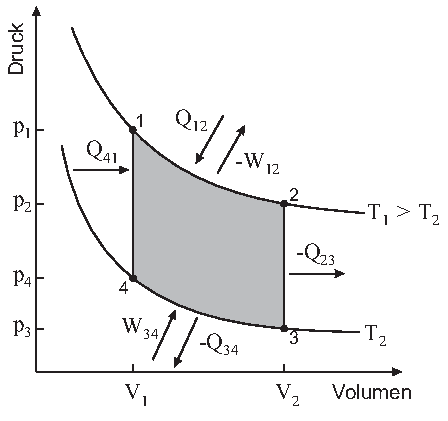
\includegraphics[width=\linewidth]{res/Stirling-Kreisprozess.pdf}
	\end{minipage}
	\begin{minipage}{0.62\linewidth}
		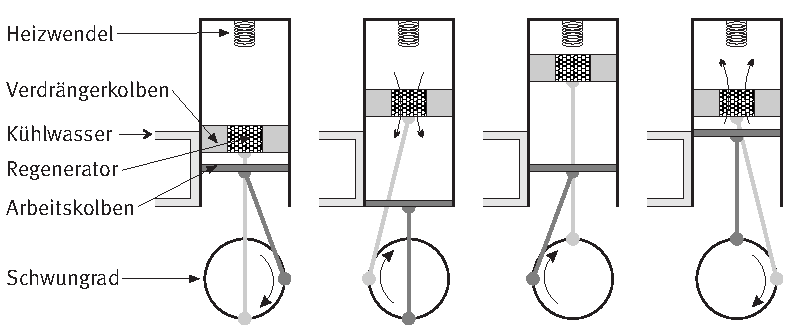
\includegraphics[width=\linewidth]{res/Takte_Stirlingmotor.pdf}
	\end{minipage}	
	\caption{Der idealisierte Stirling-Kreisprozess im $(p, V)$-Diagramm (links) und die Realisierung des Motors (rechts) mit den einzelnen Zustandsänderungen $1$ bis $4$ von links nach rechts.\cref{anleitung-ss2014} \label{fig:stirling-kreisprozess}}
\end{figure}

Eine Wärmekraftmaschine wird durch Zufuhr von Wärme betrieben und wandelt diese in nutzbare Arbeit um. Man definiert ihren Wirkungsgrad $\eta$ als Verhältnis von geleisteter Arbeit zur zugeführten Wärme. Kältemaschinen und Wärmepumpen sind "rückwärts" betriebene Wärmekraftmaschinen. Unter Aufwendung von Arbeit wird Wärme von einem kälteren Reservoir in ein wärmeres übertragen. Die Leistungszahl $\epsilon$ einer Kältemaschine ist das Verhältnis von übertragener Wärme zu aufgewandter Arbeit.
\begin{equation}\label{eq:wirkungsgrad_leistungszahl}
	\eta = \frac{\abs{W_\text{ab}}}{\abs{Q_\text{zu}}} < 1, \qquad
	\epsilon = \frac{\abs{Q_\text{ab}}}{\abs{W_\text{zu}}}
\end{equation}
Die Leistungszahl kann größer als $1$ sein.

%Wärmekraftmaschinen, Kältemaschinen und Wärmepumpen arbeiten mit einem thermodynamischen Kreisprozess, um kontinuierlich Arbeit zu leisten bzw. Wärme zu übertragen. Die entsprechenden Zustandsänderungen des Prozesses können in einem $(p, V)$-Diagramm dargestellt werden.
In \cref{fig:stirling-kreisprozess} ist der Stirling-Kreisprozess abgebildet, der aus zwei isochoren und zwei isothermen Zustandsänderungen besteht. In der Durchlaufrichtung von $1$ bis $4$ handelt es sich um eine Wärmekraftmaschine: Dem System wird
%(durch eine Heizwendel)
Wärme zugeführt und es leistet and den entsprechenden Stellen im Kreisprozess Arbeit. Im $(p, V)$-Diagramm entspricht die pro Zyklus verrichtete Arbeit wegen \cref{eq:arbeit_allgemein} der von der Kurve eingeschlossene Fläche. Soll der Kreisprozess in entgegengesetzter Richtung durchlaufen werden, muss das System
%(z.B. durch einen Motor)
angetrieben werden. Dann wird Wärme vom kälteren ins wärmere Reservoir befördert und der Stirling-Motor wird (je nachdem, welches der beiden Reservoirs betrachtet wird) als Kältemaschine bzw. Wärmepumpe betrieben.

In \cref{fig:stirling-kreisprozess} (rechts) ist der Stirling-Motor als Kolbenmaschine und Heißluftmotor umgesetzt. Das Arbeitsgas ist Luft; der Bereich um die Heizwendel ist das Reservoir höherer Temperatur ($T_1$), während der untere Bereich mit Kühlwasser gekühlt wird ($T_2$). Zwei Kolben, der Arbeitskolben und der Verdrängerkolben, sind zwischen den Reservoirs angebracht und über Pleuelstangen um \SI{90}{\degree} versetzt an einem Schwungrad befestigt. Der Arbeitskolben komprimiert die Luft bzw. lässt sie expandieren, d.h. %er verrichtet Arbeit oder
an ihm wird Arbeit verrichtet. Der Verdrängerkolben dient dazu, die Luft jeweils im richtigen Moment mit dem wärmeren oder kälteren Reservoir in Kontakt zu bringen. An ihm wird keine Arbeit verrichtet, da er das Volumen nicht ändert. Im Verdrängerkolben befindet sich zusätzlich Kupferwolle (der "Regenerator"), die durch Speicherung und Abgabe von Wärme beim Durchströmen der Luft den Wirkungsgrad erhöht.

Der Kreisprozess verläuft im Detail wie folgt:
\begin{description}
	\item[Isotherme Expansion (1 \textrightarrow\ 2):] Die Luft nimmt die Wärme $Q_{12}$ von der Heizwendel auf, dehnt sich (isotherm bei $T_1$) aus und drückt den Arbeitskolben unter Verrichtung der Arbeit $-W_{12}$ nach unten.
	\item[Isochore Abkühlung (2 \textrightarrow\ 3):] Bei der Bewegung um den unteren Tiefpunkt bewegt sich der Arbeitskolben fast nicht, d.h. $\Delta W \approx 0$. Der Verdrängerkolben bewegt die Luft, die dabei die Wärme $-Q_{23}$ an den Regenerator abgibt, nach unten.
	\item[Isotherme Kompression (3 \textrightarrow\ 4):] Das Schwungrad bewegt den Arbeitskolben nach oben, sodass dieser die Luft (bei $T_2$) komprimiert. Die Wärme $-Q_{34}$ wird an das Kühlwasser abgegeben.
	\item[Isochore Erwärmung (4 \textrightarrow\ 1):] Wie bei 2 \textrightarrow\ 3 wird (fast) keine Arbeit verrichtet. Der Verdrängerkolben bewegt die kalte Luft nach oben, die dabei die Wärme $Q_{41}$ vom Regenerator aufnimmt.
\end{description}

\section{Durchführung}
\subsection{Reibungsverluste}
Beim Betrieb als Kältemaschine entzieht der Motor der Luft pro Zyklus eine bestimmte Wärmemenge $Q_2$ und führt dem Kühlwasser die Wärme $-Q_1$ zu. Dazu muss er mit der Arbeit $-W$ angetrieben werden. Außerdem gibt es Reibungsverluste $W_R$. Die Energiebilanz für einen Umlauf lautet also
\begin{equation}\label{eq:energiebilanz}
	W = Q_1 - Q_2 + W_R
\end{equation}

Die Reibungsverluste wurden im ersten Versuchsteil bestimmt. Der Zylinderkopf des Stirling-Motors wurde dabei geöffnet und mit einem Elektromotor mit einer Frequenz $f$ von ca. \SI{3}{\Hz} angetrieben, sodass jener sich im Leerlauf befand. Die genaue Betriebsfrequenz wurde mithilfe eines Drehwinkelmessers bestimmt. Dazu wurde ca. eine Minute lang der Verlauf der Winkelposition mit einer Abtastrate von \SI{20}{\Hz} gemessen und dann die Frequenz mittels FFT ("Fast Fourier Transform") im Programm DataStudio ermittelt.

Da sich der Stirling-Motor im Leerlauf befand, wurde an das Kühlwasser nur die durch Reibung dissipierte Wärme abgegeben. Der Temperaturanstieg des Kühlwassers wurde mit einem Thermometer gemessen. Um die Reibungswärme eines Umlaufs des Motors aus dem Temperaturanstieg mit \cref{eq:wärmekapazität} zu bestimmen, wurde neben der spezifischen Wärmekapazität $c$ von Wasser auch die Masse $m$ der Wassermenge, die während eines Umlaufs durch den Motor geflossen ist, benötigt. Zur Bestimmung dieser wurde der Volumendurchsatz $V' = V/t$ des Kühlwassers gemessen, denn $m = \rho V = \rho \frac{V'}{f}$. So ergab sich für die Reibungsarbeit $W_R$ pro Umlauf:
\begin{equation}\label{eq:reibungsarbeit}
W_R = \Delta Q = c_\text{Wasser} m \Delta T
= c_\text{Wasser} \rho_\text{Wasser} \frac{V'}{f} \Delta T
\end{equation}

\subsection{Kühlleistung der Kältemaschine}
Der Stirlingmotor wurde als nächstes als Kältemaschine betrieben, indem ein Reagenzglas mit destilliertem Wasser (ca. \SI{1}{\ml}) in den Zylinder eingesetzt wurde, sodass dieser verschlossen war. Der Elektromotor betrieb den Stirling-Motor mit der gleichen Frequenz wie bei der Messung der Reibungsverluste (also ca. \SI{3}{\Hz}) und der Temperaturverlauf des Wassers mit der Zeit wurde gemessen, bis die Temperatur etwa \SI{-25}{\celsius} erreichte. (die Abtastrate wurde auf \SI{5}{\Hz} gesetzt). Aus dem Verlauf der Kurve konnten die Kühlleistung (übertragene Wärme pro Umlauf) und die Schmelzwärme des Wassers bestimmt werden. Die Kühlleistung wurde etwa bei Raumtemperatur bestimmt, da so der Einfluss der zusätzlichen Heizleistung durch die Raumluft minimiert wurde.

Außerdem wurden die Temperatur des abfließenden Kühlwassers und die des Kühlwassers im Reservoir gemessen, da aus dieser Temperaturdifferenz wieder die dem Kühlwasser zugeführte Wärme berechnet werden konnte. Aus den beiden Werten für die übertragenen Wärmebeträge pro Umlauf konnte schließlich die Leistungszahl $\epsilon$ mit \cref{eq:wirkungsgrad_leistungszahl} bestimmt werden.

\subsection{Heizleistung der Wärmepumpe}
Zum Betrieb als Wärmepumpe wurde der Elektromotor im zum vorherigen Versuch umgekehrten Drehsinn eingeschaltet. Die Drehzahl wurde weiterhin beibehalten. Wie bei der Kältemaschine wurden Temperaturverlauf des Wassers (Beginn bei \SI{-25}{\celsius}) und Temperaturanstieg des Kühlwassers gemessen. So konnten analog zur Kältemaschine Heizleistung und Leistungszahl der Wärmepumpe bestimmt werden. Die spezifische Wärme von Eis konnte ebenfalls aus dem Temperaturverlauf gefolgert werden.

\subsection{Wirkungsgrad der Wärmekraftmaschine}
Der Stirling-Motor wurde nun als Wärmekraftmaschine betrieben, d.h. der Elektromotor wurde entfernt und stattdessen eine Heizwendel in den Zylinder eingesetzt. Der Stirling-Motor trieb nun selbst das Rad an.

Im ersten Versuchsteil wurde die Heizleistung und der Wirkungsgrad (unbelastet) mithilfe des $(p, V)$-Diagramms ermittelt. Dazu wurde der Motor bei Heizspannungen von ca. \SIlist{8; 10; 12; 14; 16}{\V} betrieben. Der Druck im Stirlingmotor und ein an den Kolben angeschlossenes Drehwinkel-Messgerät wurden dafür jeweils mit einer Abtastrate von \SI{1}{\kHz} gemessen. Die Winkelposition war proportional zum Volumen der Luft im Motor. Dem minimalen und dem maximalen Drehwinkel aus den Messwerten ($\phi_\text{min}$ bzw. $\phi_\text{max}$) entsprachen die Werte für das maximale Volumen $V_\text{max} = \sagestr{SI(195+140,0,'cm^3')}$ und minimale Volumen $V_\text{min} = \SI{195}{\cm^3}$. Da der Zusammenhang linear ist, konnten mit einer Geradengleichung durch Einsetzen des Wertepaars $V_\text{max}, \phi_\text{min}$ und $V_\text{min}, \phi_\text{max}$ Steigung und Achsenabschnitt bestimmt werden.Deshalb wurde die Winkelposition wie folgt in das Volumen umgerechnet:
\begin{equation}\label{eq:volumen_umrechnung}
\begin{aligned}
V(\phi) &= m \phi + b = \frac{\Delta V}{\Delta \phi} + b
= \frac{V_\text{max} - V_\text{min}}{\phi_\text{min} - \phi_\text{max}} + b\\
b &= V_\text{max} - \frac{\Delta V}{\Delta \phi} \phi_\text{min} = V_\text{min} - \frac{\Delta V}{\Delta \phi} \phi_\text{max}
\end{aligned}
\end{equation}

Es wurde für jede Messung die jeweilige Heizspannung eingestellt und der Motor konnte wurde für einige Minuten warmlaufen. Die erzeugte Frequenz wurde durch Messung der Winkelposition (ca. \SI{1}{min} lang) und FFT bestimmt. Führ die zugeführte Heizleistung wurden die gemessenen Werte von Stromstärke und Spannung bei der Heizwendel verwendet. Die Stromstärke wurden dabei mit einem Induktionsdraht bestimmt. Dieser wurde dreimal um das Kabel gewickelt; so entsprachen \SI{3}{\mV} gemessene Spannung einer Stromstärke von \SI{1}{\A}.

Im zweiten Teil wurde der belastete Stirling-Motor mit dem Pronyschen Zaum untersucht. Die Heizspannung war konstant bei ca. \SI{16}{\V}. Der Zaum wurde am Schwungrad befestigt, sodass dieses abgebremst wurde. Die Leistung des Motors ließ sich bestimmen, indem mit einer Federwaage die vom Zaum ausgeübte Kraft $F$ gemessen wurde:
\begin{equation}\label{eq:prony}
P = 2 \pi f M = 2 \pi f F r
\end{equation}
Dabei ist $r$ die Länge von der Mitte des Zaums bis zum Angreifpunkt der Federwaage. Die Messung wurde für $12$ Werte von $f$ durchgeführt. Es wurde der Wirkungsgrad gegen die Frequenz dargestellt und so das Wirkungsgradmaximum ermittelt.





\section[Auswertung]{Auswertung%
\footnote{Die ermittelten Messwerte sind im Laborbuch zu finden.
Die in der Auswertung angegebenen Unsicherheiten auf den Ergebnissen wurden bei direkter Messung aus dem abgeschätzten systematischen Fehler und (bei mehreren Messungen) dem statistischen Fehler und bei berechneten Größen mit der Fehlerfortpflanzung bestimmt (s. \cref{sec:fehlerrechnung}).
Bei der grafischen Auswertung wurden die Abbildungen, berechneten Parameter und zugehörige Unsicherheiten
durch gnuplot \autocite{gnuplot} bestimmt.}}

\nocite{sage}


%Volumendurchsatz
\begin{sagesilent}
V(ml_1, ml_2, ml_3, s_1, s_2, s_3) = 1/3*(ml_1/s_1+ml_2/s_2+ml_3/s_3)
delta_V = gauss_error(V)

Volumen = V(91, 95, 99, 21.75, 23, 23.75)
Volumen_err = delta_V(91, 95, 99, 21.75, 23, 23.75,1, 1, 1, 0.05, 0.05, 0.05)
Volumen_ausgabe = SI(Volumen.n(digits=4),Volumen_err.n(digits=2),'ml/s')
\end{sagesilent}



%Reibungsarbeit
\begin{sagesilent}
W_R(c_w, roh, V_, f, delta_T) = c_w*roh*V_*delta_T/f
delta_W_R = gauss_error(W_R)

Reibungsarbeit = W_R(4.182, 1,Volumen, 3, 0.5)
Reibungsarbeit_err = delta_W_R(4.182, 1,Volumen, 3,0.5,0.005,0,Volumen_err, 0,0.1)
Reibungsarbeit_ausgabe = SI(Reibungsarbeit,Reibungsarbeit_err,'J', digits=2)
\end{sagesilent}

%Q1 Abkühlung 
\begin{sagesilent}
Q(c_w, roh, V_, f, delta_T) = c_w*roh*V_*delta_T/f
delta_Q = gauss_error(Q)

Abkuehlung = Q(4.182, 1,0.9, 3, 0.5)
Abkuehlung_err = delta_Q(4.182, 1,0.9, 3,0.5,0.005,0,0.1, 0,0.1)
Abkuehlung_ausgabe = SI(Abkuehlung,Abkuehlung_err,'J', digits=3)
\end{sagesilent}



%Kühleistung bei Raumtemperatur
\begin{sagesilent}
P(c_w,m_w,m)=c_w*m_w*m
delta_P=gauss_error(P)

Kuehlleistung = P(4.182,0.9,-0.1768695)
Kuehlleistung_err = delta_P(4.182,0.9,-0.1768695,0,0.2,0.0028408)
Kuehlleistung_ausgabe = SI(Kuehlleistung, Kuehlleistung_err,'W', digits=2)
\end{sagesilent}


%Kühlleistung bei 0 °C 
\begin{sagesilent}
P(c_w,m_w,m)=c_w*m_w*m
delta_P=gauss_error(P)

KuehlleistungBeiNull = P(4.182,0.9,-0.12087412)
KuehlleistungBeiNull_err = delta_P(4.182,0.9,-0.12087412,0,0.2,0.0001564458)
KuehlleistungBeiNull_ausgabe = SI(KuehlleistungBeiNull.n(digits=3), KuehlleistungBeiNull_err.n(digits=2),'W')
\end{sagesilent}


%Q2 Abkühlen
\begin{sagesilent}
Q2(P, f)=P/f
delta_Q2=gauss_error(Q2)

Abkuehlung2 = Q2(Kuehlleistung, 3)
Abkuehlung2_err = delta_Q2(Kuehlleistung, 3, Kuehlleistung_err,0)
Abkuehlung2_ausgabe = SI(Abkuehlung2.n(digits=3), Abkuehlung2_err.n(digits=3),'J')
\end{sagesilent}




%Schmelzwärme
\begin{sagesilent}
Q(P,t)=P*t
delta_Q=gauss_error(Q)

schmelzwaerme = -Q(Kuehlleistung,320.8)
schmelzwaerme_err = delta_Q(Kuehlleistung,320.8,Kuehlleistung_err,20)
schmelzwaerme_ausgabe = SI(schmelzwaerme,schmelzwaerme_err,'J', digits=2)
\end{sagesilent}

%Leistungszahl Abkühlen
\begin{sagesilent}
epsilon(Q, Q2, W_R) = abs(Q2)/abs(abs(Q)-abs(Q2)+abs(W_R))
delta_epsilon = gauss_error(epsilon)

leistungszahl = epsilon(Abkuehlung, Abkuehlung2, Reibungsarbeit)
leistungszahl_err = delta_epsilon(Abkuehlung, Abkuehlung2, Reibungsarbeit, Abkuehlung_err, Abkuehlung2_err, Reibungsarbeit_err)
leistungszahl_ausgabe = SI(leistungszahl, leistungszahl_err, digits=3)
leistungszahl_ausgabe_prozent = SI(leistungszahl*100, leistungszahl_err*100, '\\%', digits=1)
\end{sagesilent}

%Heizleistung bei Raumtemperatur
\begin{sagesilent}
P_H(c_w,m_w,m) = c_w*m_w*m
delta_P_H = gauss_error(P_H)

Heizleistung = P_H(4.182, 0.9, 0.3590726)
Heizleistung_err = delta_P_H(4.182, 0.9, 0.3590726, 0.005, 0.1, 0.003004129)

Heizleistung_ausgabe = SI(Heizleistung, Heizleistung_err, 'W', digits=2)
\end{sagesilent}



%Heizleistung bei -10 bis -8 °C
\begin{sagesilent}
P_H(c_w,m_w,m) = c_w*m_w*m
delta_P_H = gauss_error(P_H)

HeizleistungUnterNull = P_H(4.182, 0.9, 0.60371517)
HeizleistungUnterNull_err = delta_P_H(4.182, 0.9, 0.60371517, 0.005, 0.1, 0.0067934)

HeizleistungUnterNull_ausgabe = SI(HeizleistungUnterNull, HeizleistungUnterNull_err, 'W', digits = 2)
\end{sagesilent}




%spezifische Wärme von Eis
\begin{sagesilent}
c_E(c_W,m_W,m_E) = c_W*m_W/m_E
delta_c_E= gauss_error(c_E)

spezifische_Waerme = c_E(4.182, 0.35907258, 0.60371517)
spezifische_Waerme_err = delta_c_E(4.182,  0.35907258, 0.60371517, 0.005, 0.00304129, 0.0067934)

spezifische_Waerme_ausgabe = SI(spezifische_Waerme, spezifische_Waerme_err, 'J/(gK)', digits = 2)
\end{sagesilent}

%Q1 Erhitzen
\begin{sagesilent}
Q(c_e, roh, V_, f, delta_T) = c_e*roh*V_*delta_T/f
delta_Q = gauss_error(Q)

Erhitzen = Q(spezifische_Waerme, 0.9, 0.9, 3, 0.6)
Erhitzen_err = delta_Q(spezifische_Waerme, 1,0.9, 3,0.6,spezifische_Waerme_err,0.1, 0.1, 0,0.1)

Erhitzen_ausgabe = SI(Erhitzen, Erhitzen_err, 'J', digits = 2)
\end{sagesilent}



%Q2 Erhitzen
\begin{sagesilent}
Q2(P, f)=P/f
delta_Q2=gauss_error(Q2)

Erhitzen2 = Q2(Heizleistung, 3)
Erhitzen2_err = delta_Q2(Heizleistung, 3, Heizleistung_err,0)

Erhitzen2_ausgabe = SI(Erhitzen2, Erhitzen2_err,'J', digits=2)
\end{sagesilent}


%Leistungszahl Erhitzen
\begin{sagesilent}
epsilon(W_R, Q1, Q2) = abs(Q2)/abs(abs(Q1)-abs(Q2)+abs(W_R))
delta_epsilon = gauss_error(epsilon)

Wirkung = epsilon(Reibungsarbeit, Erhitzen, Erhitzen2)
Wirkung_err = delta_epsilon(Reibungsarbeit, Erhitzen, Erhitzen2, Reibungsarbeit_err, Erhitzen_err, Erhitzen2_err)

Wirkung_ausgabe = SI(Wirkung, Wirkung_err, digits = 2)
Wirkung_ausgabe_prozent = SI(Wirkung*100, Wirkung_err*100, ' \\%', digits = 1)
\end{sagesilent}


\subsection{Kältemaschine}
Zunächst wurde der Volumendurchsatz des Kühlwassers gemessen. Dieser betrug\\$\sagestr{Volumen_ausgabe}$. Die Temperatur des Kühlwassers stieg von $\SI{20.3}{°C}$ um $\SI{0.5}{°C}$ auf $\SI{20.8}{°C}$. Das entspricht nach \cref{eq:reibungsarbeit} einer Reibungsarbeit pro Umlauf von $\sagestr{Reibungsarbeit_ausgabe}$.

\begin{figure}
	\centering
	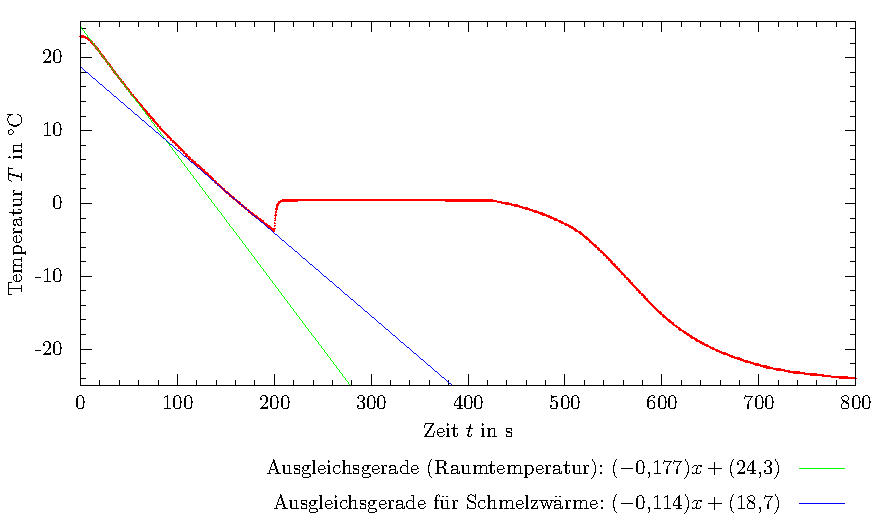
\includegraphics{res/Kuehlleistung.tex}
	\caption{Kühltemperatur $T$ in Abhängigkeit von der Zeit $t$ (Abkühlen). \label{Kühlleistung}}
\end{figure}


In \cref{Kühlleistung} sind deutlich die verschiedenen Phasen des Abkühlungsprozesses zu erkennen. Zu Beginn gibt es einen nahezu linearen Abfall auf ca. $\SI{-4}{°C}$. Da es sich um destilliertes Wasser handelt und somit Kristallisationskeime fehlen, fällt die Temperatur sogar unter $\SI{0}{°C}$. Es folgt ein Sprung auf $\SI{0}{°C}$, bei dem die Temperatur für einige Zeit $(\SI{220+-10}{s})$ stagniert. In dieser Phase wird dem Wasser weiter Energie entzogen, bis es in den festen Zustand überführt werden kann. Anschließend sinkt die Temperatur weiter ab bis auf $\SI{-24}{°C}$. 

Die Kühlleistung $P_K$ der Kältemaschine wurde mithilfe einer Ausgleichsgerade und \cref{eq:wärmekapazität} bestimmt. Sie liegt bei
$P_K = \sagestr{Kuehlleistung_ausgabe}$.

Die Schmelzwärme des Wassers konnte mit der Kühlleistung um den Gefrierpunkt (bestimmt aus einer weiteren Ausgleichsgerade) und der Dauer des Gefrierprozesses (s.o.) bestimm werden. Für destilliertes Wasser liegt die gemessene Schmelzwärme $\Delta Q$ bei $\sagestr{schmelzwaerme_ausgabe}$.

Aus der pro Umlauf an das Kühlwasser abgegebenen Wärme $Q_1 = \sagestr{Abkuehlung_ausgabe}$, der dem destillierten Wasser pro Umlauf entzogenen Wärme $Q_2 = \sagestr{Abkuehlung2_ausgabe}$ und der Reibungsarbeit $W_R = \sagestr{Reibungsarbeit_ausgabe}$
ergibt die Leistungszahl der Kältemaschine $\epsilon_K = \sagestr{leistungszahl_ausgabe} = \sagestr{leistungszahl_ausgabe_prozent}$


\subsection{Wärmepumpe}
Die Heizleistung $P_K$ der Wärmepumpe wurde wie die Kühlleistung zuvor mithilfe einer Ausgleichsgerade bestimmt. Sie liegt bei $P_K = 
\sagestr{Heizleistung_ausgabe}$ und ist somit deutlich höher als die Kühlleistung des gleichen Stirling-Motors. 

In \cref{Heizleistung} sind wie bei der Kältemaschine die unterschiedlichen Phasen des Erwärmungsprozesses zu erkennen. Die Temperatur steigt annähernd linear bis ca \SI{0}{°C} an und verbleibt für einige Zeit bei dieser Temperatur. Es wird Energie aufgenommen, die das Eis für den Schmelzprozess benötigt. Da die Heizleistung der Wärmepumpe höher ist als die Kühlleistung der Kältemaschine, ist diese Phase bei der Wärmepumpe schon nach ca. \SI{150+-10}{s}, und somit \SI{70}{s} schneller als bei der Kältemaschine, vorbei. Anschließend folgt ein abflachender Anstieg auf eine Temperatur von \SI{70}{°C}. Dieser wird durch die Raumtemperatur beeinflusst; bis \SI{20}{°C} steigt die Temperatur schneller als im restlichen Verlauf, da die Raumtemperatur bis dahin eine zusätzliche Heizleistung auf das Wasser ausübt.

\begin{figure}
	\centering
	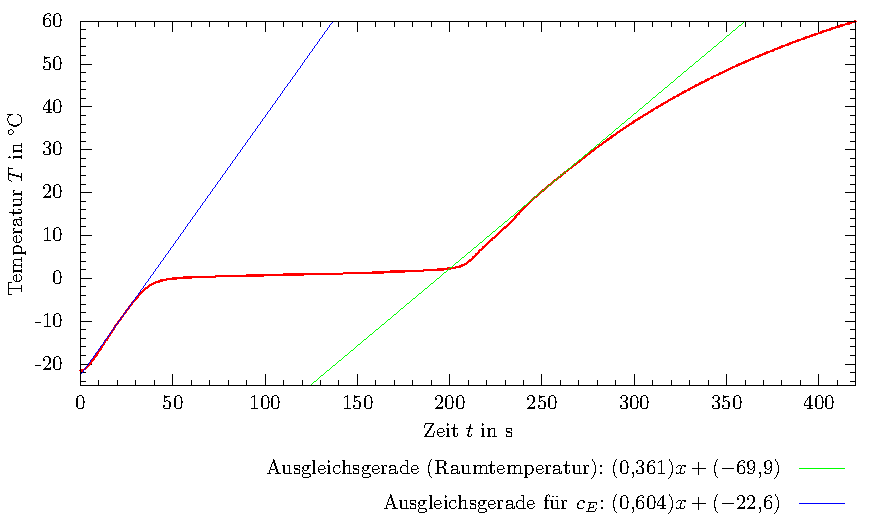
\includegraphics{res/Heizleistung.tex}
	\caption{Erhitzungstemperatur $T$ in Abhängigkeit von der Zeit $t$ (Erhitzen). \label{Heizleistung}}
\end{figure}


Aus der dem Kühlwasser zugeführten Wärme $Q_1 = \sagestr{Erhitzen_ausgabe}$ und der dem destillierten Wasser zugeführten Wärme $Q_2 = \sagestr{Erhitzen2_ausgabe}$ sowie der Reibungsarbeit ergibt die Leistungszahl der Wärmepumpe $\epsilon_W =  \sagestr{Wirkung_ausgabe} = \sagestr{Wirkung_ausgabe_prozent}$. Die Leistungszahl der Wärmepumpe ist ca. doppelt so hoch wie die der Kältemaschine.

Für die spezifische Wärme von Eis wurde der vom Motor erzeugte Temperaturanstieg pro Sekunde in der festen Phase mit dem in der flüssigen verglichen. Da der Motor dem Wasser die gleiche Leistung zuführt, ist der Unterschied auf die Wärmekapazitäten zurückzuführen: $c_W m \Delta T_W = c_E m \Delta T_E$. Die spezifische Wärme von Eis wurde so auf $c_E = \sagestr{spezifische_Waerme_ausgabe}$ bestimmt.


\subsection{Wirkungsgrad aus dem $(p, V)$-Diagramm}
\begin{sagesilent}
V_min = 195			# cm^3
V_max = V_min + 140	# cm^3
\end{sagesilent}
Wie in der Durchführung beschrieben wurde der Stirling-Motor mit einer Heizwendel als Wärmekraftmaschine betrieben. Für verschiedene Heizspannungen $U_H$ wurde die Heizleistung bestimmt, das $(p, V)$-Diagramm gezeichnet und so der Wirkungsgrad der Wärmekraftmaschine berechnet. Da das Vorgehen für jeden Wert der Heizspannung gleich ist, wird es einmal (für  $U_H = \SI{8}{\V}$) ausführlich erläutert und für die weiteren Werte nur verkürzt dargestellt.

\subsubsection{Betrieb mit \SI{8}{\V}}
\begin{sagesilent}
phi_min = -0.335	# rad
phi_max = 1.684		# rad

m = (V_max - V_min)/(phi_min - phi_max)
b = V_max - m * phi_min
m_print = SI(m, 0, r'\cm\cubed\per\radian')
b_print = SI(b, 0, r'\cm\cubed')

I_o = 19666.9253508156	# kPa * cm^3 = 10^(-3) J = mJ
I_u = 18406.3569793955	# kPa * cm^3 = 10^(-3) J = mJ
W = (I_o - I_u) / 1000	# J
W_err = 0.05			# J
I_o_print = SI(I_o, 0, r'm\J', digits=2)
I_u_print = SI(I_u, 0, r'm\J', digits=2)
W_print = SI(W, W_err, r'\J', digits=2)

U = 7.4					# V
I = 0.028 * 1000 / 3	# A
P(U_, I_) = U_ * I_
delta_P = gauss_error(P)
P_H = P(U, I)						# W
P_H_err = delta_P(U, I, 0.1, 1/3)	# W
U_print = SI(U, 0.1, r'\V', digits=2)
I_print = SI(I, 1/3, r'\A', digits=2)
P_H_print = SI(P_H, P_H_err, '\\W', digits=1)

f = 3.477000		# Hz
f_err = 0.021573	# Hz
f_print = SI(f, f_err, r'\Hz', digits=2)

Q(P_H_, f_) = P_H_/f_
delta_Q = gauss_error(Q)
waerme_zu = Q(P_H, f)
waerme_zu_err = delta_Q(P_H, f, P_H_err, f_err)
waerme_zu_print = SI(waerme_zu, waerme_zu_err, r'\J', digits=2)

eta(W_, Q_) = abs(W_)/abs(Q_)
delta_eta = gauss_error(eta)
wirkungsgrad = eta(W, waerme_zu)
wirkungsgrad_err = delta_eta(W, waerme_zu, W_err, waerme_zu_err)
wirkungsgrad_print = SI(wirkungsgrad, wirkungsgrad_err, digits=3)
wirkungsgrad_prozent_print = SI(wirkungsgrad*100, wirkungsgrad_err*100, r'\percent', digits=1)
\end{sagesilent}

\begin{figure}
	\centering
	\includegraphics{res/8V-p,v.tex}
	\caption{$(p, V)$-Diagramm für $U_H = \SI{8}{V}$. \label{fig:wk_8V}}
\end{figure}
In \cref{fig:wk_8V} ist die Auswertung der Messwerte für das $(p, V)$-Diagramm bei einer Heizspannung von ca. \SI{8}{\V} zu sehen. Zunächst musste für die Skalierung der $V$-Achse die gemessene Winkelposition mit \cref{eq:volumen_umrechnung} in das entsprechende Volumen umgerechnet werden: 
\begin{align*}
\phi_\text{min} &= \sagestr{SI(phi_min, 0, 'rad')} \\
\phi_\text{max} &= \sagestr{SI(phi_max, 0, 'rad')} \\
\implies V(\phi) &= \sagestr{m_print} \cdot \phi + \sagestr{b_print}
\end{align*}
Um die pro Umlauf geleistete Arbeit zu berechnen, musste die von der Kurve in \cref{fig:wk_8V} eingeschlossene Fläche bestimmt werden. Dazu wurde wie folgt vorgegangen: Die obere und die untere "Hälfte" der Kurve wurden voneinander getrennt, mittels eines Fit je eine Funktion für beide Kurvenhälften ermittelt und beide Funktionen von $V_\text{min}$ bis $V_\text{max}$ integriert. Der Wert des jeweiligen Integrals ist die Fläche unter der jeweiligen Kurvenhälfte. Die Differenz des oberen und des unteren Integrals ist damit die gesuchte eingeschlossene Fläche, d.h. die pro Umlauf vom Motor verrichtete Arbeit.

Um die Kurvenhälften zu trennen, wurde mit gnuplot eine "Trennkurve" ermittelt. Ein Fit der Form $\sfrac{a}{V} + b$ und geringefügige manuelle Modifikationen des Ergebnisses lieferten in allen Fällen eine geeignete Trennkurve, die zwischen oberer und unterer Hälfte verlief. Alle Punkte oberhalb der Trennkurve wurden zur oberen, alle unterhalb zur unteren Hälfte gezählt.

Da beim Stirling-Kreisprozess (\cref{fig:stirling-kreisprozess}) ein ideales Gas angenommen wurde, würde man nach \cref{eq:zustandsgleichung} für die Isothermen einen Verlauf der Kurvenhälften $\sim \sfrac{1}{V}$ erwarten. Wie aber bereits in \cref{fig:wk_8V} zu sehen ist, folgt der reale Stirling-Motor nicht diesem idealisierten Verlauf. Die Kurvenhälften wurden deshalb jeweils mit einem Polynom 6. Grades approximiert (die ermittelten Parameter sind in den Abbildungen zu finden).

Die Integration ergab die folgenden Ergebnisse für die obere ($I_o$) und untere ($I_u$) Kurve:
\begin{align*}
I_o &= \sagestr{I_o_print} \\
I_u &= \sagestr{I_u_print} \\
\implies \abs{W} &= I_o - I_u = \sagestr{W_print}
\end{align*}
Der Fehler des Flächeninhalts wurde dabei nach Betrachtung der Abbildung mit 50 Flächeneinheiten ($= \SI{50}{m\\J}$) abgeschätzt.

Zur Bestimmung des Wirkungsgrads wurden noch die elektrische Leistung $P_H$ der Heizwendel und die Frequenz $f$ des Motors bestimmt. Mit den gemessenen Werten für die Stromstärke und Spannung ergab sich für die Heizleistung:
\begin{equation*}
P_H = U_H I_H = \sagestr{U_print} \cdot \sagestr{I_print} = \sagestr{P_H_print}
\end{equation*}

Die Frequenz wurde aus dem Frequenzspektum (FFT) auf $f = \sagestr{f_print}$ bestimmt. Als Fehler wurde die Halbwertsbreite im Frequenzspektrum der FFT gewählt. Die entsprechenden Abbildungen (die ansonsten keinen Zweck erfüllen) wurden aus Gründen der Übersichtlichkeit nicht in das Protokoll aufgenommen. Die pro Umlauf zugeführte Wärme $Q$ errechnete sich so zu
\begin{equation*}
Q = \frac{P_H}{f} = \sagestr{waerme_zu_print}
\end{equation*}

Mit \cref{eq:wirkungsgrad_leistungszahl} ergab sich für den Wirkungsgrad
\begin{equation*}
\eta = \frac{\abs{W}}{\abs{Q}} = \sagestr{wirkungsgrad_print} = \sagestr{wirkungsgrad_prozent_print}
\end{equation*}


\newcommand{\pv}[1]{
	\subsubsection{Betrieb mit \SI{#1}{\V}}
	\begin{figure}
		\centering
		\includegraphics{res/#1V-p,v.tex}
		\caption{$(p, V)$-Diagramm für $U_H = \SI{#1}{V}$. \label{fig:wk_#1V}}
	\end{figure}
	In \cref{fig:wk_#1V} ist die Auswertung der Messwerte für das $(p, V)$-Diagramm bei einer Heizspannung von ca. \SI{#1}{\V} zu sehen. Zunächst musste für die Skalierung der $V$-Achse die gemessene Winkelposition mit \cref{eq:volumen_umrechnung} in das entsprechende Volumen umgerechnet werden:
	\begin{align*}
	\phi_\text{min} &= \sagestr{phi_min_print[#1]} \\
	\phi_\text{max} &= \sagestr{phi_max_print[#1]} \\
	\implies V(\phi) &= \sagestr{m_print[#1]} \cdot \phi + \sagestr{b_print[#1]}
	\end{align*}
	
	Die Integration ergab die folgenden Ergebnisse für die obere ($I_o$) und untere ($I_u$) Kurve:
	\begin{align*}
	I_o &= \sagestr{I_o_print[#1]} \\
	I_u &= \sagestr{I_u_print[#1]} \\
	\implies \abs{W} &= I_o - I_u = \sagestr{W_print[#1]}
	\end{align*}
	
	Mit den gemessenen Werten für die Stromstärke und Spannung ergab sich für die Heizleistung:
	\begin{equation*}
	P_H = U_H I_H = \sagestr{U_print[#1]} \cdot \sagestr{I_print[#1]} = \sagestr{P_H_print[#1]}
	\end{equation*}
	
	Die Frequenz wurde %aus \cref{fig:fft_#1v}
	auf $f = \sagestr{f_print[#1]}$ bestimmt. Die pro Umlauf zugeführte Wärme $Q$ errechnete sich so zu
	\begin{equation*}
	Q = \frac{P_H}{f} = \sagestr{waerme_zu_print[#1]}
	\end{equation*}
	
	Mit \cref{eq:wirkungsgrad_leistungszahl} ergab sich für den Wirkungsgrad
	\begin{equation*}
	\eta = \frac{\abs{W}}{\abs{Q}} = \sagestr{wirkungsgrad_print[#1]} = \sagestr{wirkungsgrad_prozent_print[#1]}
	\end{equation*}
}

\begin{sagesilent}
#				 10V				12V					14V			16V
data = {
	'phi_min' : (-2.015,			-1.704,				-0.066,		-0.759),
	'phi_max' : (0.006,				0.327,				1.967,		1.28),
	'I_o'	  : (20099.4420446203,	20624.99521747,		21320.4451,	21205.0067621293),
	'I_u'	  : (18350.8530705003,	18325.8087508654,	17976.597,	17819.9655516904),
	'U'		  : (9.1,				11.0,				13.3,		14.6),
	'I'		  : [x*1000/3 for x in \
				  (0.033,			0.038,				0.044,		0.048)],
	'f'		  : (5, 				6.289,				7.5,		8.359),
	'f_err'	  : (0.030917,			0.038555,			0.035862,	0.023781),
}
m_print, b_print, I_o_print, I_u_print, W_print, U_print, I_print, P_H_print, f_print, waerme_zu_print, wirkungsgrad_print, wirkungsgrad_prozent_print, phi_min_print, phi_max_print = (dict(), dict(), dict(), dict(), dict(), dict(), dict(), dict(), dict(), dict(), dict(), dict(), dict(), dict())

for idx, volts in enumerate((10, 12, 14, 16)):
  phi_min = data['phi_min'][idx]
  phi_max = data['phi_max'][idx]
  I_o = data['I_o'][idx]
  I_u = data['I_u'][idx]
  W = (I_o - I_u) / 1000
  W_err = 0.05
  U = data['U'][idx]
  I = data['I'][idx]
  f = data['f'][idx]
  f_err = data['f_err'][idx]
  
  m = (V_max - V_min)/(phi_min - phi_max)
  b = V_max - m * phi_min
  P_H = P(U, I)						# W
  P_H_err = delta_P(U, I, 0.1, 1/3)	# W
  
  phi_min_print[volts] = SI(phi_min, 0, r'\radian')
  phi_max_print[volts] = SI(phi_max, 0, r'\radian')
  
  m_print[volts] = SI(m, 0, r'\cm\cubed\per\radian')
  b_print[volts] = SI(b, 0, r'\cm\cubed')
  
  I_o_print[volts] = SI(I_o, 0, r'm\J', digits=2)
  I_u_print[volts] = SI(I_u, 0, r'm\J', digits=2)
  W_print[volts] = SI(W, W_err, r'\J', digits=2)
  
  U_print[volts] = SI(U, 0.1, r'\V', digits=2)
  I_print[volts] = SI(I, 1/3, r'\A', digits=2)
  P_H_print[volts] = SI(P_H, P_H_err, r'\W', digits=1)
  
  f_print[volts] = SI(f, f_err, r'\Hz', digits=2)
  
  waerme_zu = Q(P_H, f)
  waerme_zu_err = delta_Q(P_H, f, P_H_err, f_err)
  waerme_zu_print[volts] = SI(waerme_zu, waerme_zu_err, r'\J', digits=2)
  
  wirkungsgrad = eta(W, waerme_zu)
  wirkungsgrad_err = delta_eta(W, waerme_zu, W_err, waerme_zu_err)
  wirkungsgrad_print[volts] = SI(wirkungsgrad, wirkungsgrad_err, digits=3)
  wirkungsgrad_prozent_print[volts] = SI(wirkungsgrad*100, wirkungsgrad_err*100, r'\percent', digits=1)
\end{sagesilent}

\pv{10}

\pv{12}

\pv{14}

\pv{16}

\subsection{Wirkungsgrad mit Abbremsen}
\begin{figure}
	\centering
	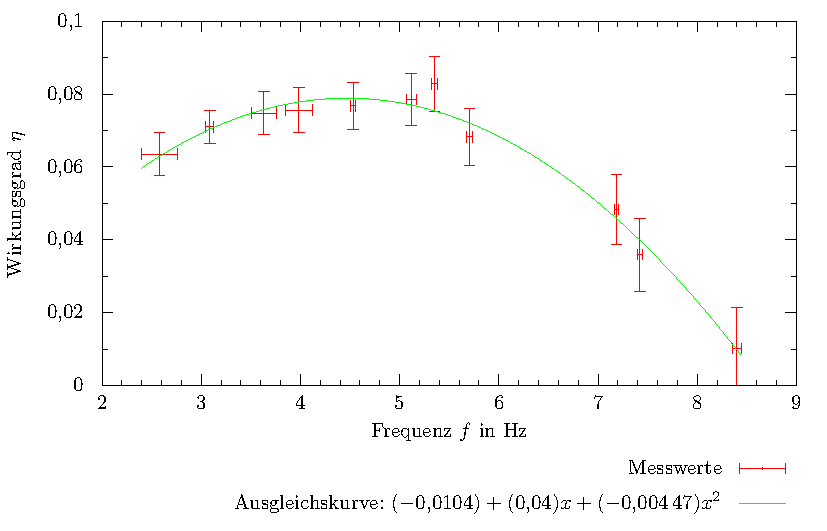
\includegraphics{res/prony.tex}
	\caption{Gemessene Wirkungsgrade und Motorfrequenzen beim Betrieb unter Last mit dem Pronyschen Zaum. \label{fig:prony}}
\end{figure}
Die Messungen mit dem Pronyschen Zaum wurden wie in der Durchführung beschrieben durchgeführt. Es wurde sowohl die Leistung des Motors mit \cref{eq:prony} als auch die elektrische Heizleistung gemessen. Bei der letzteren waren für alle Messungen $U = \SI{14.6 +- 0.2}{\V}$ und $I = \sagestr{SI(0.048*1000/3, 1/3, r'\A', digits=1)}$, d.h. $P_\text{el} = \sagestr{SI(P(14.6, 0.048*1000/3), delta_P(14.6, 0.048*1000/3, 0.2, 1/3), r'\W', digits=1)}$. Die Ergebnisse sind in \cref{fig:prony} zu sehen. Der Wirkungsgrad wurde analog zu \cref{eq:wirkungsgrad_leistungszahl} berechnet: $\eta = \sfrac{\abs{W}}{\abs{Q}} = \sfrac{P}{P_\text{el}}$.

Ebenfalls abgebildet ist eine quadratische Ausgleichskurve, da die Messwerte einem parabelförmigen Verlauf zu folgen scheinen. Identifiziert man das Maximum der Ausgleichskurve mit dem Wirkungsgradmaximum, so liegt dieses bei
\begin{align*}
\eta_\text{max} &= \num{0.0791} = \SI{7.91}{\%}\\
f_\text{max} &= \SI{4.47}{\Hz}
\end{align*}


\section{Diskussion}
Bei der Bestimmung der Kühlleistung für die Kältemaschine war es wichtig, das Verhältnis $\Delta T/\Delta t$ bei Raumtemperatur zu messen, da sonst die von der Raumluft übertragene Wärme ebenfalls einen Einfluss haben würde.

Bei der Bestimmung der Schmelzwärme von destilliertem Wasser liegt der Literaturwert bei $\SI{334}{\J}$)\footcite[S. 636]{taschenbuch}. Der gemessene Wert weicht vom Literaturwert ab, was dadurch bedingt ist, dass der Stirling-Motor nicht komplett von der Umgebung abgeschlossen ist und somit noch Wärme von außen hinzu kommt. Eine weitere Fehlerquelle könnte die geringe Menge des Wassers sein: Zum einen ist die so mögliche Ungenauigkeit relativ hoch, zum anderen kühlt der Motor neben dem Wasser z.B. auch die Luft im Reagenzglas und das Glas selbst. Aufgrund der geringen Wassermenge könnten diese Einflüsse eine starke Auswirkung haben.

Bei der Bestimmung der spezifischen Wärme von Eis wurde eine Temperatur von $T = \SI{-9}{°C}$ vorausgesetzt, da im Bereich von ca. $\SI{-3}{°C}$ bis $\SI{2}{°C}$ die Kurve stark abfällt und somit die Werte dadurch verfälscht werden können. Der berechnete Wert stimmt innerhalb des Messfehlers mit dem Literaturwert von ($\SI{2.1}{J/(gK)}$)\footcite[S. 630]{taschenbuch} überein. Auch hier sind Abweichungen durch den von der Umgebung schlecht isolierten Stirling-Motor und Nebeneffekte des Versuchsaufbaus zu erklären.

Bei der Bestimmung des Wirkungsgrades des Stirling-Motors als Wärmekraftmaschine mithilfe der $(p, V)$-Diagramme entsprachen die Ergebnisse den Erwartungen. Die entstandenen Diagramme haben alle eine dem idealen Stirling-Prozess angenäherte, "bananenförmige" Gestalt. Das Druckminimum liegt bei allen Heizspannungen bei einem ähnlichen Wert, während das Maximum aufgrund der schnelleren Bewegung des Kolbens bei höheren Spannungen etwas ansteigt. Mit zunehmender Heizleistung nimmt auch die Fläche im $(p, V)$-Diagramm, also die Leistung des Motors, zu. Da dem Motor mehr Energie zugeführt wird, kann er auch mehr Arbeit verrichten. Die einzige auffällige Abbildung ist \cref{fig:wk_14V}, bei der eine relativ hohe Streuung der Messpunkte auftritt. Da der Tisch, auf dem der Motor stand, während des Versuchs stark wackelte, liegt die Vermutung nahe, dass bei dieser Frequenz des Motors der Tisch zu besonders starken Schwingungen angeregt wurde und so dessen Verhalten beeinflusst hat.

Die Wirkungsgrade nahmen mit zunehmender Heizspannung von \SI{6,3}{\%} bei \SI{8}{\V} bis mehr als \SI{12}{\%} bei \SIlist{14; 16}{\V} zu. Am höchsten war der Wirkungsgrad bei \SI{14}{\V}, sodass dort ein Wirkungsgradmaximum für den unbelasteten Motor vorliegen könnte. Allerdings liegt der Wert bei \SI{16}{\V} im Bereich der Messunsicherheit, sodass es sich sich auch um eine messbedingte Abweichung handeln könnte.

Bei der Bestimmung des Wirkungsgrads mit dem Pronyschen Zaum schienen die Werte einem parabelförmigen Verlauf zu folgen. So konnte aus einer Ausgleichskurve das Wirkungsgradmaximum des belasteten Motors auf 
\SI{7.91}{\%} ($f = \SI{4.47}{\Hz}$) bestimmt werden. Ein einzelner Punkt bei ca. \SI{5,5}{\Hz} lag relativ weit über der Kurve (dort lag das Maximum der tatsächlich gemessenen Werte). Allerdings lässt sich aufgrund der starken Abweichung vom Verlauf der restlichen Punkte sagen, dass es sich vermutlich um einen Messfehler handelt. Der Zaum musste z.B. immer parallel zum Boden liegen, damit das Drehmomentgleichgewicht nach \cref{eq:prony} gilt. Mit bloßem Augenmaß lässt die Genauigkeit dort zu wünschen übrig, sodass Abweichungen entstehen können.